\subsection{DMS pathway inhibition does not impact virtual corridor navigation}
\label{sec:glmhmm:2.2.2}


\begin{figure}[t!]
  \begin{center}
    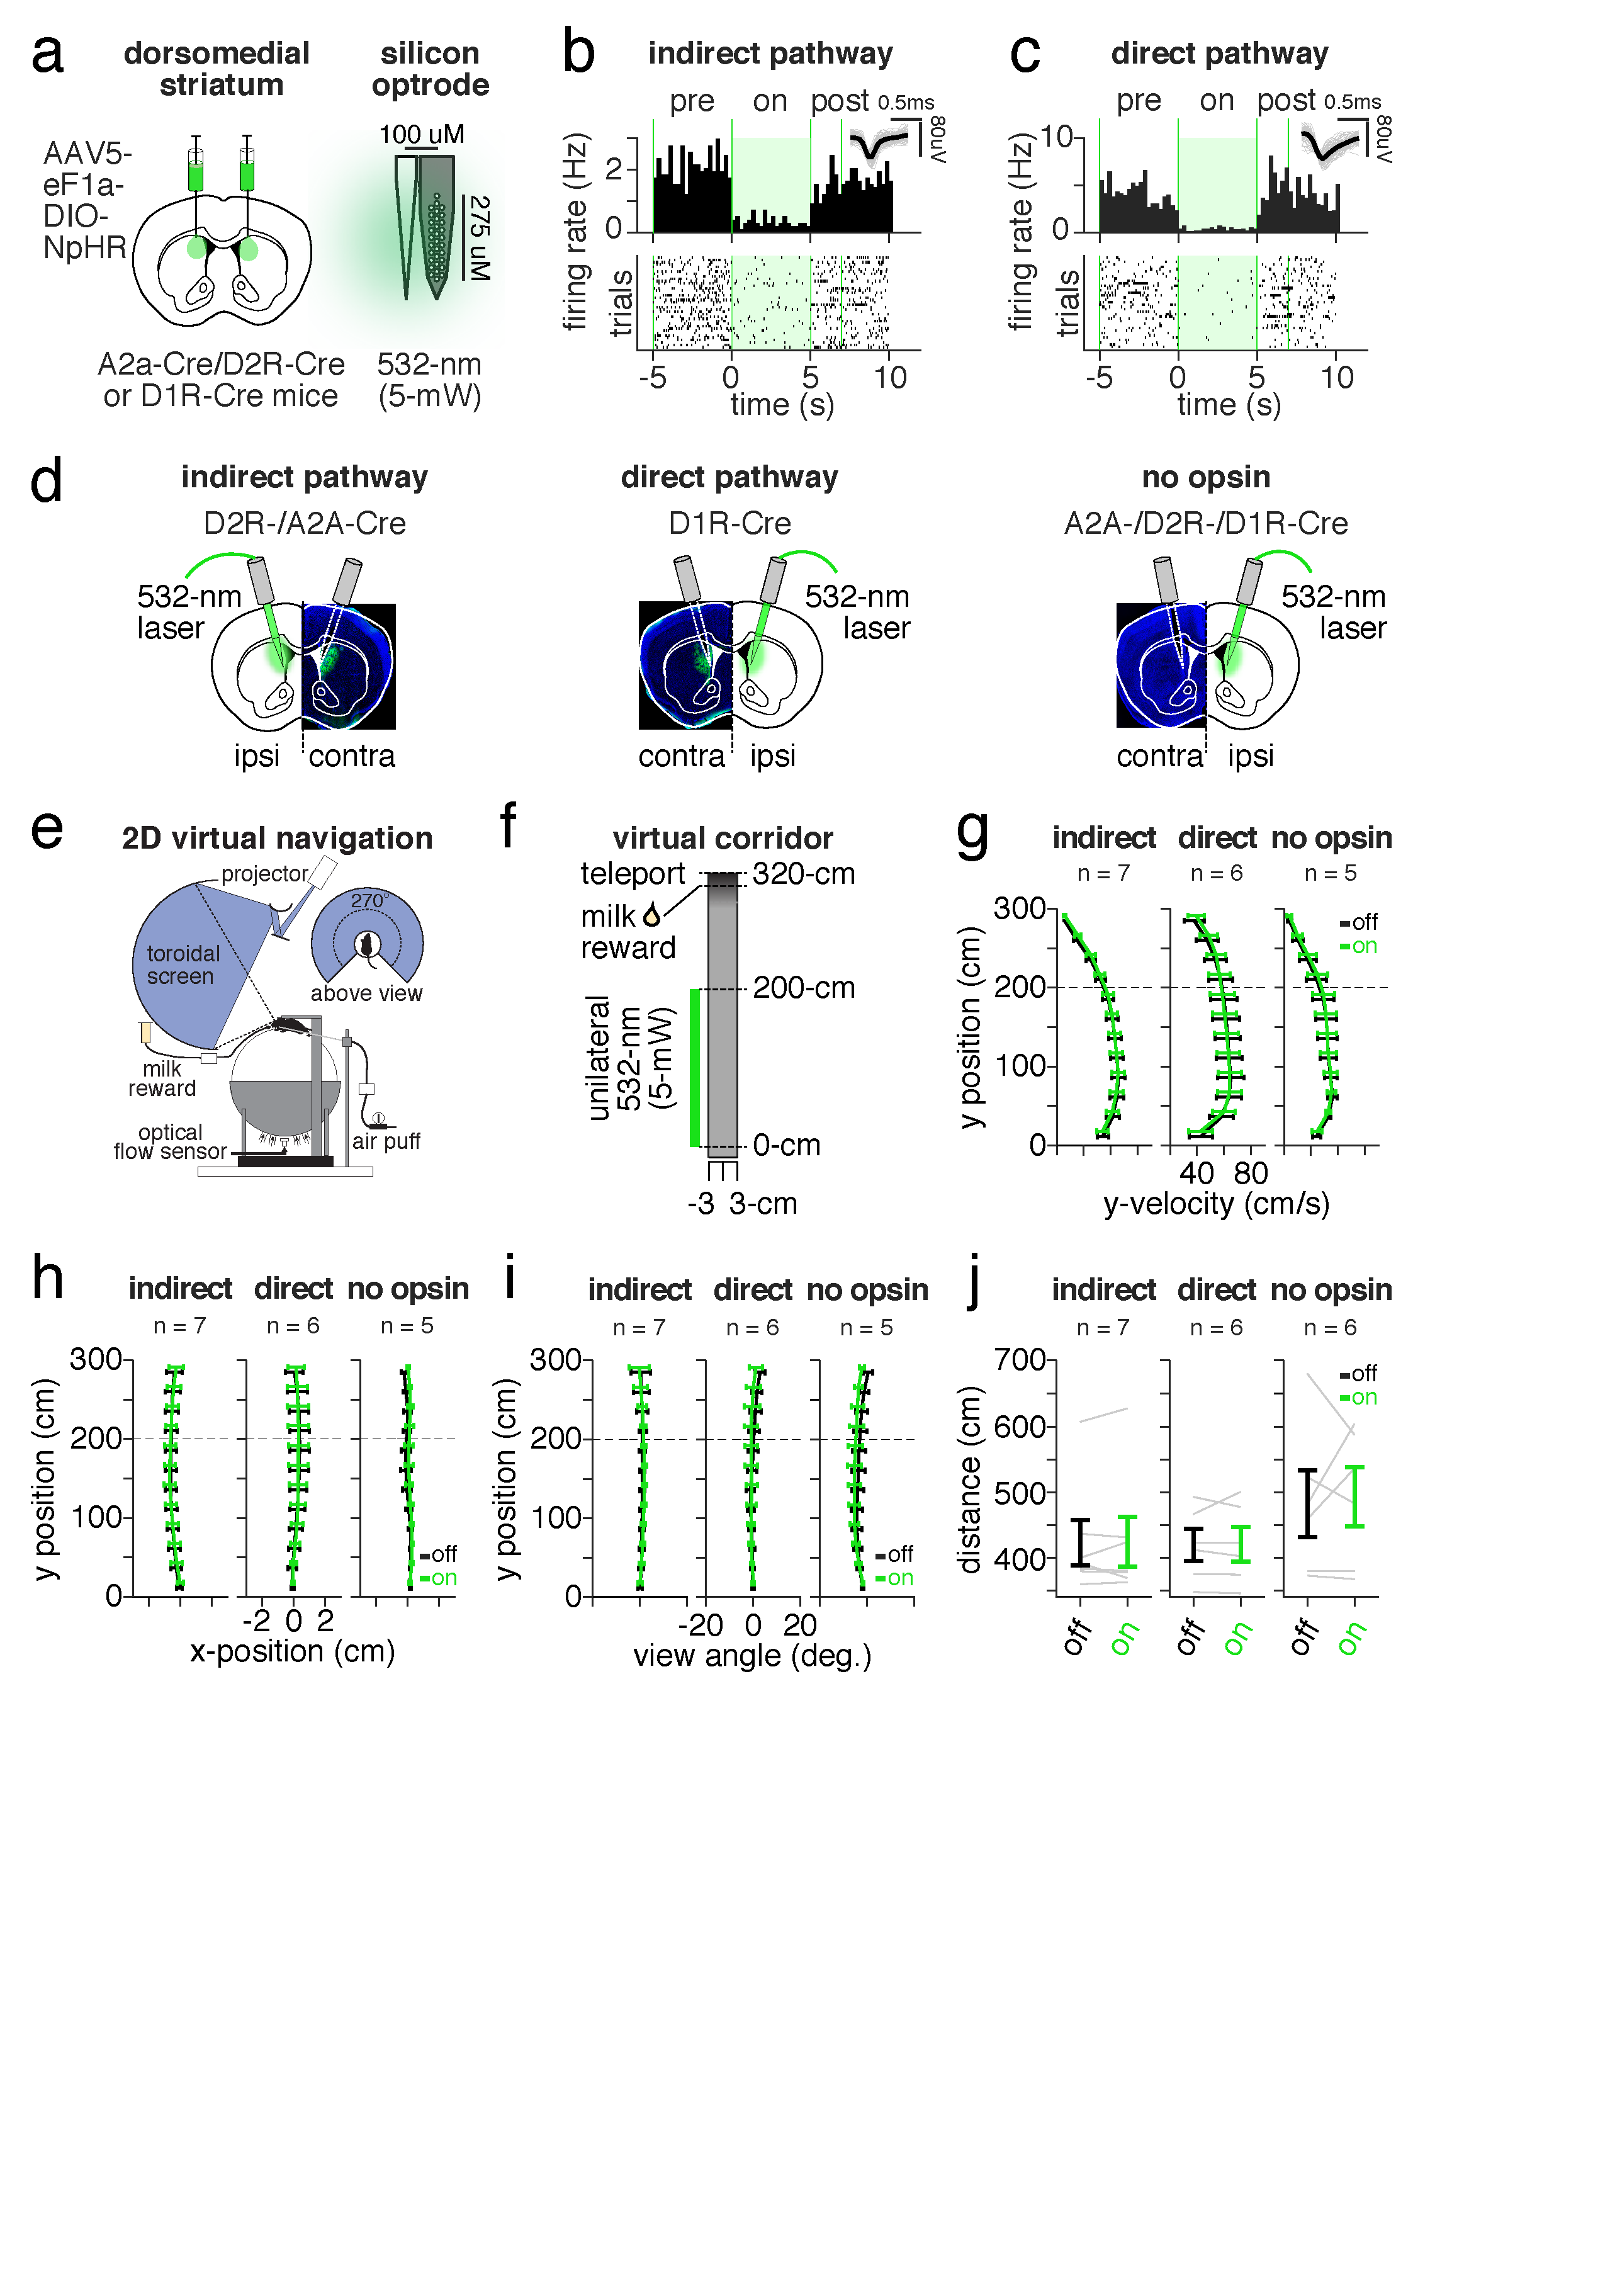
\includegraphics[width=0.90\linewidth]{ch2-glmhmm/glmhmm-figures/Fig1.pdf}
    \caption[Pathway-specific DMS inhibition has no detectable impact on movement in mice navigating a virtual corridor]{\textbf{Pathway-specific DMS inhibition has no detectable impact on movement in mice navigating a virtual corridor.} (a) Schematic of viral delivery of Cre-dependent halorhodopsin (NpHR) to the dorsomedial striatum (DMS) of A2a-Cre, D2R-Cre, or D1R-Cre mice (left). Schematic of optrode (right): a 32-channel silicon probe coupled with tapered optical fiber, which delivered 532-nm (5-mW) light to the DMS of awake, ambulating mice. (b) Example peristimulus time histograms (PSTH) (top) and rasters of trial-by-trial spike times (bottom) from a DMS single-unit recorded in an ambulating A2a-Cre mouse expressing Cre-dependent NpHR (indirect pathway). Inset: average spike waveform (black) and 100 randomly sampled spike waveforms (grey). A trial consisted of 5-s without laser (pre, -5 to 0-s), 5-s laser sweep (on, 0 to 5-s), and 10-s ITI (40 total trials). (c) As in b but for DMS single-unit in a D1R-Cre mouse expressing}
    \label{fig:glmhmm:1}
  \end{center}
  \vspace{-1.5cm}
\end{figure}
\begin{figure}[t!]
  \contcaption{Cre-dependent NpHR (direct pathway). (d) Schematic of bilateral fiberoptic implantation of DMS and unilateral illumination in behaving mice, with example histology from a mouse expressing NpHR in the indirect (left, D2R-/A2a-Cre) or direct (middle, D1R-Cre) pathways, or control mouse without opsin (right, no opsin, A2a-/D2R- or D1R-Cre). 532-nm light (5-mW) was delivered unilaterally to the left or right hemisphere on alternate testing sessions and lateralized behavior was defined as ipsilateral or contralateral relative to the laser hemisphere. (e) Schematic of head-fixation of mice in a virtual reality (VR) apparatus allowing 2-D navigation. Displacements of an air-suspended spherical ball in the anterior-posterior (and medial-lateral) axes of the mouse controlled y- (and x-) position movements in a visual VR environment. (f) Schematic of virtual corridor 6-cm in width and 330-cm in length, consisting of a start region (-10-0cm), an inhibition region (0-200cm) in which mice received unilateral 532-nm light on a random subset of trials (30\%), a reward location (310cm) where mice received reward, and a teleportation location (320cm) where mice were transported to the start region following a variable ITI with mean of 2-s. (g) Average y-velocity (cm/s) across mice as a function of y-position (0-300cm in 25-cm bins) while navigating the virtual corridor on laser off (black) or laser on (green) trials in groups receiving DMS indirect (left, n = 7 mice, n = 1,712 laser off and n = 1,288 laser on trials) or direct pathway inhibition (middle, n = 6 mice, n = 1,088 laser off and n = 757 laser on trials), or illumination of the DMS in the absence of NpHR expression (right, no opsin, n = 5 mice, n = 1,178 laser off and n = 827 laser on trials). (h) Same as g but for average x-position (cm) contralateral to the unilaterally-coupled laser hemisphere. (i) Same as g but for view angle (degrees, contralateral to laser hemisphere). (j) Average across-mouse distance travelled (cm) to traverse the virtual corridor during laser off (black) or laser on (green) trials for mice receiving DMS indirect (n = 7 mice, n = 2,109 laser off and n = 1,574 laser on trials) or direct pathway inhibition (n = 6 mice, n = 1,330 laser off and n = 930 laser on trials), or DMS illumination in the absence of NpHR (n = 6  mice, n = 1,688 laser off and n = 1,199 laser on trials). Solid bars depict mean $\pm$S.E.M. across mice; grey lines indicate individual mouse mean.}% Continued caption
\end{figure}

To determine if endogenous activity in DMS pathways provides bidirectional control of motor output in the absence of a decision, we carried out unilateral inhibition of indirect and direct pathways in head-fixed mice running on an air-supported ball to traverse a 2-dimensional linear corridor in virtual reality (VR) (Fig. \ref{fig:glmhmm:1}d-f, 6-cm x 330-cm corridor). Illumination of the DMS was restricted to 0-200cm (laser on 30\% of trials; hemisphere of illumination alternated across days). The parameters of the virtual corridor and inhibition period were selected to closely match the stem of the VR-based T-maze decision-making tasks that are the focus of subsequent experiments.

We found no detectable impact of pathway-specific DMS inhibition, nor DMS illumination alone, on multiple indicators of motor output during virtual corridor navigation. This included measures of velocity, x-position or view angle relative to the laser hemisphere, and distance traveled (Fig. \ref{fig:glmhmm:1}g-j; see Extended Data Fig. \ref{fig:ap1:ext2} for additional measures). Similarly, we obtained null effects of pathway-specific inhibition on velocity (and spatial preference) in freely behaving mice in a conditioned place preference assay (Supplementary Fig. \ref{fig:ap1:supp3}). 

These negative findings argue against a major involvement of endogenous activity in DMS pathways in the execution of movement in the absence of a decision. This is consistent with the dearth of reports demonstrating strong and opposing modulation of behavior by striatal pathways using pathway-specific optogenetic inhibition. 
